\documentclass[12pt]{article}
\usepackage[margin=1.25in]{geometry}
\usepackage[svgnames,x11names,table]{xcolor}
\usepackage{hyperref}
\usepackage{graphicx}
\usepackage{parskip}
\usepackage{float}
\usepackage{amsmath}
\usepackage{amssymb}
\usepackage{enumitem}
\usepackage[thicklines]{cancel}

\usepackage{pgfplots}
\pgfplotsset{compat=1.17}

\hypersetup{
    colorlinks,
    citecolor=black,
    filecolor=black,
    linkcolor=RoyalBlue4,
    urlcolor=RoyalBlue4,
}

\title{PEU 323 Assignment 4}
\author{Mohamed Hussien El-Deeb (201900052)}
\date{}

\begin{document}

\renewcommand{\labelenumi}{\textbf{(\alph{enumi})}}

\maketitle
\tableofcontents
\newpage
\section{Problem 1}

 (a) Yes, this wave function is physically acceptable if the normalization constant \( A \) is chosen such that \(\int_{-a}^{a} |\psi(x)|^2 \, dx = 1\). The wave function is continuous and single-valued within \([-a, a]\), meeting the requirements for physical acceptability.

\begin{figure}[H]
    \centering
    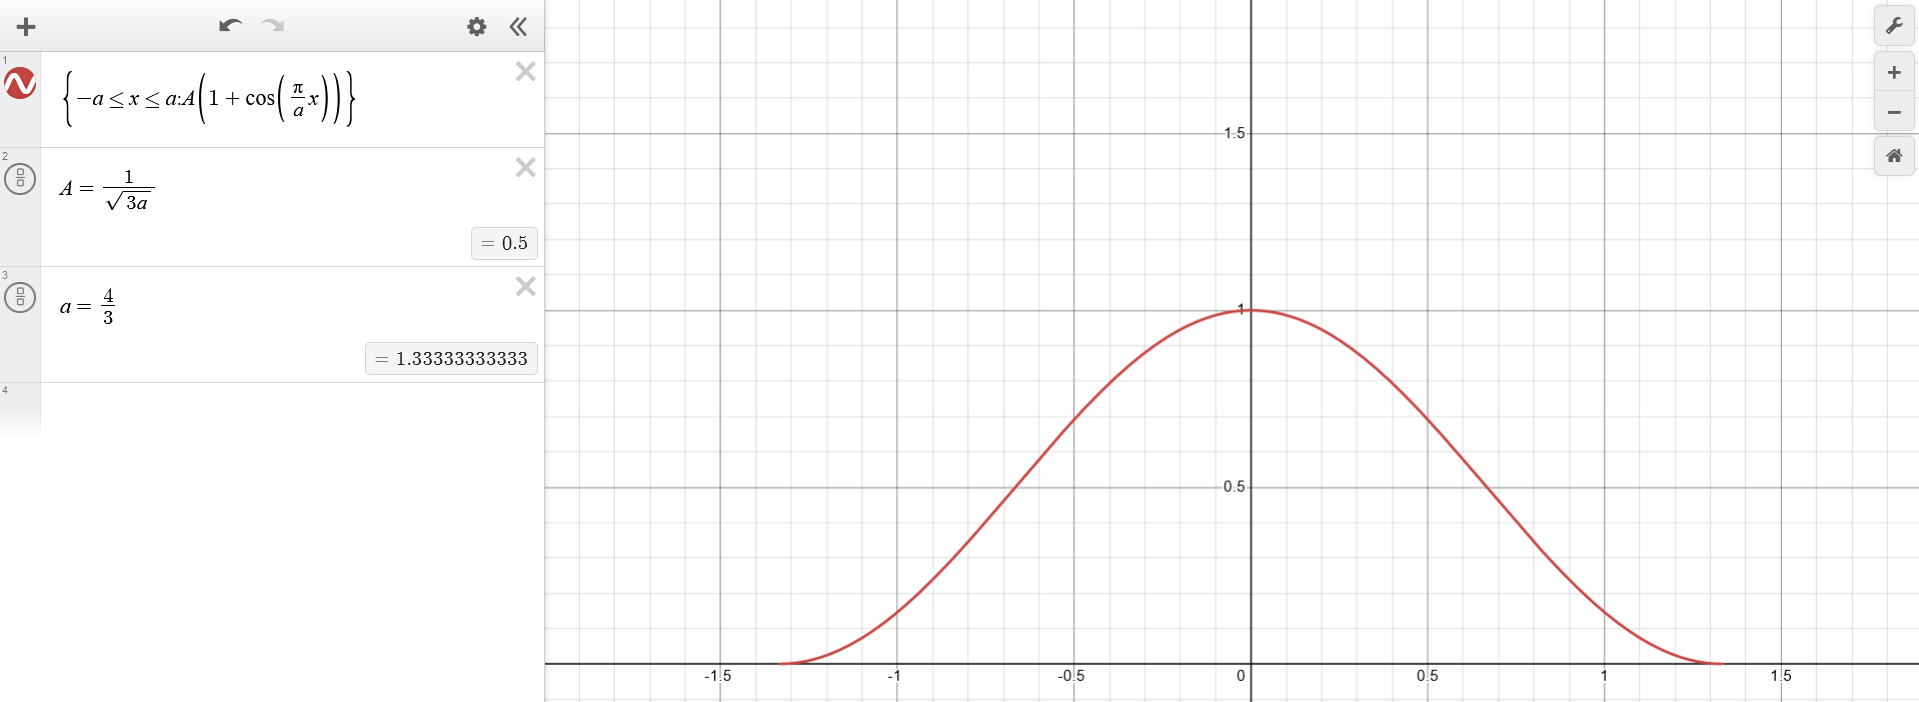
\includegraphics[width=0.7\linewidth]{Q1.png}
    \caption{$\psi$}
\end{figure}

(b) The classically allowed region is:

\[
    [-a, a]
\]

since the wave function \(\psi(x) = 0\) outside this interval, meaning the classical particle cannot be found outside \([-a, a]\).

\newpage
\section{Problem 2}

\begin{enumerate}
    \item
          \[
              \psi(x, t) = \sin \left( \frac{n \pi}{a} x \right) e^{-i \omega t}
          \]



          \[
              \frac{-\hbar^2}{2m}
              \frac{\partial^2 \psi}{\partial x^2} + V(x) \psi = i\hbar \frac{\partial \psi}{\partial t}
          \]

          \begin{equation*}
              \begin{split}
                  V(x) \psi
                    & = \frac{\hbar^2}{2m}
                  \frac{\partial^2 \psi}{\partial x^2}
                  + i\hbar \frac{\partial \psi}{\partial t}                                                                    \\
                    & = \frac{\hbar^2}{2m}
                  \frac{\partial^2 (\sin \left( \frac{n \pi}{a} x \right))}{\partial x^2}e^{-i \omega t}
                  + i\hbar \sin \left( \frac{n \pi}{a} x \right) \frac{\partial (e^{-i \omega t})}{\partial t}                 \\
                    & = - \frac{\hbar^2 n^2 \pi^2}{2ma^2} \sin\left( \frac{n \pi}{a} x \right) e^{-i \omega t}
                  + \omega \hbar \sin \left( \frac{n \pi}{a} x \right) e^{-i \omega t}                                         \\
                    & = (\omega \hbar - \frac{\hbar^2 n^2 \pi^2}{2ma^2}) \sin \left( \frac{n \pi}{a} x \right) e^{-i \omega t} \\
                    & = (\omega \hbar - \frac{\hbar^2 n^2 \pi^2}{2ma^2}) \psi                                                  \\
                  V & = \omega \hbar - \frac{\hbar^2 n^2 \pi^2}{2ma^2}
              \end{split}
          \end{equation*}

    \item

          To find the expectation value \(\langle x \rangle\), we observe that the term \(\sin^2 \left( \frac{n \pi}{a} x \right)\) is symmetric around \(x = \frac{a}{2}\). By shifting the domain of \(\psi(x)\) as \(\psi(x) \rightarrow \psi \left( x - \frac{a}{2} \right)\), we redefine the domain as \(-\frac{a}{2} \leq x \leq \frac{a}{2}\).

          Under this transformation, the shifted wave function becomes an even function, while \(x\) (as a variable) is odd with respect to \(x = 0\). As a result, the integrand for \(\langle x' \rangle = \int_{-\frac{a}{2}}^{\frac{a}{2}} x' |\psi(x')|^2 \, dx'\) is an odd function over a symmetric interval, leading to:

          \[
              \langle x' \rangle = 0.
          \]

          To obtain \(\langle x \rangle\) in the original coordinates, we perform the inverse transformation \(x' = x - \frac{a}{2}\), which implies \(x = x' + \frac{a}{2}\). Thus:

          \[
              \langle x \rangle = \langle x' + \frac{a}{2} \rangle = \langle x' \rangle + \frac{a}{2} = 0 + \frac{a}{2} = \frac{a}{2}.
          \]

          Therefore, the average position of the particle is:

          \[
              \langle x \rangle = \frac{a}{2}.
          \]

\end{enumerate}
\newpage
\section{Problem 3}
Fourier transform:
\[
    \phi(k) = \frac{1}{\sqrt{2\pi}} \int_{-\infty}^{\infty} \psi(x) e^{-ikx} \, dx
\]
Inverse Fourier transform:
\[
    \psi(x) = \frac{1}{\sqrt{2\pi}} \int_{-\infty}^{\infty} \phi(k) e^{ikx} \, dk
\]

\[
    \langle p \rangle = \int_{-\infty}^{\infty} \psi^*(x) \left( -i \hbar \frac{d}{dx} \right) \psi(x) \, dx
\]


\[
    \langle p \rangle = \int_{-\infty}^{\infty} \int_{-\infty}^{\infty} \phi^*(k') e^{-ik'x} \, dk' \left( -i \hbar \frac{d}{dx} \right) \int_{-\infty}^{\infty} \phi(k) e^{ikx} \, dk \, dx
\]

\[
    -i \hbar \frac{d}{dx} e^{ikx} = \hbar k e^{ikx}
\]
\[
    \langle p \rangle = \int_{-\infty}^{\infty} \int_{-\infty}^{\infty} \phi^*(k') \phi(k) \hbar k \left( \frac{1}{2\pi} \int_{-\infty}^{\infty} e^{i(k - k')x} \, dx \right) dk' \, dk
\]

\[
    \frac{1}{2\pi} \int_{-\infty}^{\infty} e^{i(k - k')x} \, dx = \delta(k - k')
\]

\[
    \langle p \rangle = \int_{-\infty}^{\infty} \int_{-\infty}^{\infty} \phi^*(k') \phi(k) \hbar k \delta(k - k')\, dk' \, dk
\]

\[ \therefore
    \langle p \rangle = \int_{-\infty}^{\infty} \hbar k |\phi(k)|^2 \, dk
\]

where \(|\phi(k)|^2\) represents the probability density in \(k\)-space and \(\hbar k\) is the momentum associated with each \(k\).

\newpage
\section{Problem 4}
\begin{enumerate}
    \item
          If a system is in a pure energy eigenstate, its time evolution is given by:

          \[
              \psi(x, t) = \psi(x, 0) e^{-i E t / \hbar}
          \]

          \[
              \psi(x, t + T) = \psi(x, t)
          \]

          \[
              \psi(x, 0) e^{-i E (t+T) / \hbar}  = \psi(x, 0) e^{-i E t / \hbar}
          \]

          \[
              \therefore e^{-i E T / \hbar} = 1
          \]

          \[
              \therefore \frac{E T}{\hbar} = 2 \pi n, \quad n \in \mathbb{N}
          \]

          \[
              T = \frac{2 \pi \hbar}{E} n
          \]

    \item

          \[
              E = \frac{2 \pi \hbar}{T} n
          \]

    \item
          For a particle in an infinite square well
          \[
              E_n = \frac{n^2 \pi^2 \hbar^2}{2m L^2}
          \]

          \[
              T = \frac{2 \pi \hbar}{E_n} n = \frac{4 m}{n \pi \hbar} L^2
          \]

\end{enumerate}

\newpage
\section{Problem 5}
The wave function stays undisturbed (the same) after the sudden expansion
\[
    \psi_0 = \sqrt{\frac{2}{L}}\cos{(\frac{\pi}{L}x)}, \quad -\frac{L}{2} \leq x \leq \frac{L}{2}
\]

% \begin{equation*}
%     \psi = 
%     \begin{cases}     
%         \sqrt{\frac{2}{L}}\cos{(\frac{\pi}{L}x)}, & , \quad \text{if} -\frac{L}{2} \leq x \leq \frac{L}{2} \\
%         0,& \text{otherwise}
%     \end{cases}
% \end{equation*}

The new ground state:

\[
    \psi'_0 = \sqrt{\frac{1}{L}}\cos{(\frac{\pi}{2L}x)}, \quad -L \leq x \leq L
\]

\begin{equation*}
    \begin{split}
        \langle \psi | \psi_0' \rangle
         & = \frac{\sqrt{2}}{L} \int_{-\frac{L}{2}}^{\frac{L}{2}} \cos{(\frac{\pi}{2L}x)}\cos{(\frac{\pi}{L}x)}\,dx                                        \\
         & = \frac{\sqrt{2}}{L} \int_{-\frac{L}{2}}^{\frac{L}{2}} \cos{(\frac{\pi}{2L}x)}[1-2\sin^2{(\frac{\pi}{2L}x)}]\,dx                                \\
         & = \frac{\sqrt{2}}{L} \left[\frac{2L}{\pi}\sin{(\frac{\pi}{2L}x)} - \frac{4L}{3\pi}\sin^3{(\frac{\pi}{2L}x)}\right]_{-\frac{L}{2}}^{\frac{L}{2}} \\
         & = \frac{2\sqrt{2}}{\pi} \left[\sin{(\frac{\pi}{2L}x)} - \frac{2}{3}\sin^3{(\frac{\pi}{2L}x)}\right]_{-\frac{L}{2}}^{\frac{L}{2}}                \\
         & =  \frac{8}{3 \pi}
        % & = \frac{2\sqrt{2}}{L} \int_{-\frac{L}{2}}^{\frac{L}{2}} \sin^2{(\frac{\pi}{2L}x)}\cos{(\frac{\pi}{2L}x)}\,dx \\
        % & = \frac{4\sqrt{2}}{3 \pi} \left[\sin^3{(\frac{\pi}{2L}x)}\right]_0^{L} = 0 = \frac{4\sqrt{2}}{3 \pi}
    \end{split}
\end{equation*}

\[
    P = |\langle \psi | \psi_0' \rangle|^2 = {|\frac{8}{3 \pi}|}^2 = \frac{64}{9\pi^2}
\]

\newpage
\section{Problem 6}

\begin{enumerate}
    \item

          \begin{equation*}
              V(x) =
              \begin{cases}
                  0 \quad   & \text{if} \, -a_0 \leq x \leq -a_0 \\
                  V_0 \quad & \, otherwise                       \\
              \end{cases}
          \end{equation*}

          \[
              \text{where}\; V_0 = 20eV
          \]

          \[
              m = 9.109 \times 10^{-31} kg
          \]

          \[
              \hbar = 1.05457182 \times 10^{-34} m^2 kg / s
          \]

          \[
              a = 2a_0, \quad a_0 = 0.529 \times 10^{-10}m
          \]

          For bound states,

          \[
              0 < E < V_0
          \]

          For \(-\infty \leq x \leq -a_0,\quad a_0 \leq x \leq \infty \):

          Schrodinger equation:

          \[
              \frac{\hbar^2}{2m}\frac{\partial^2 \psi}{\partial x^2} = -(E - V_0) \psi
          \]

          %   \[
          %       \frac{-\hbar^2}{2m}\frac{\partial^2 \psi}{\partial x^2} = E \psi
          %   \]

          \[
              \frac{\partial^2 \psi}{\partial x^2} = l^2 \psi
          \]

          \[
              \text{where}\; l = \frac{\sqrt{2m (V_0 - E)}}{\hbar}
          \]

          \[
              \psi_1 = A e^{l x} + B e^{- l x}
          \]

          \[
              \psi_3 = E e^{l x} + F e^{- l x}
          \]

          For \(-a_0 \leq x \leq a_0 \):

          Schrodinger equation:

          \[
              \frac{\partial^2 \psi}{\partial x^2} = -\frac{2mE}{\hbar^2} \psi
          \]

          \[
              \frac{\partial^2 \psi}{\partial x^2} = - k^2 \psi
          \]

          \[
              \text{where}\; k = \frac{\sqrt{2m E}}{\hbar}
          \]

          \[
              \psi_2 = C \sin{(k x)} + D \cos{(k x)}
          \]

          \[
              \alpha \equiv \frac{l}{k} = \sqrt{\frac{V_0}{E} - 1},\quad \alpha > 0
          \]

          Our $\psi$ now is:

          \begin{equation*}
              \therefore
              \psi(x) =
              \begin{cases}
                  A e^{l x} + B e^{- l x} \quad       & \text{if} \, -\infty < x < -a_0   \\
                  C \sin{(k x)} + D \cos{(k x)} \quad & \text{if} \, -a_0 \leq x \leq a_0 \\
                  E e^{l x} + F e^{- l x} \quad       & \text{if} \, a_0 < x < \infty     \\
              \end{cases}
          \end{equation*}
          \begin{equation*}
              \therefore
              \psi'(x) =
              \begin{cases}
                  l (A e^{l x} - B e^{- l x}) \quad       & \text{if} \, -\infty < x < -a_0   \\
                  k (C \cos{(k x)} - D \sin{(k x)}) \quad & \text{if} \, -a_0 \leq x \leq a_0 \\
                  l (E e^{l x} - F e^{- l x}) \quad       & \text{if} \, a_0 < x < \infty     \\
              \end{cases}
          \end{equation*}

          By applying the boundary conditions:

          \[
              \psi(x = -\infty) = 0 \implies B = 0
          \]
          \[
              \psi(x = \infty) = 0 \implies E = 0
          \]
          \[
              \psi(x = -a_0) \implies A e^{- l a_0} = D \cos{(k a_0)} - C \sin{(k a_0)} \tag{1}\label{equ.1}
          \]
          \[
              \psi(x = a_0) \implies F e^{- l a_0} = C \sin{(k a_0)} + D \cos{(k a_0)} \tag{2}\label{equ.2}
          \]
          \[
              \psi'(x = -a_0) \implies A e^{- l a_0} = \frac{k}{l} (C \cos{(k a_0)} + D \sin{(k a_0)}) \tag{3}\label{equ.3}
          \]
          \[
              \psi'(x = a_0) \implies F e^{- l a_0} = \frac{k}{l} (D \sin{(k a_0)} - C \cos{(k a_0)}) \tag{4}\label{equ.4}
          \]

          \[
              \begin{pmatrix}
                  e^{- l a_0} & \sin{(k a_0)}               & -\cos{(k a_0)}             & 0           \\
                  e^{- l a_0} & - \frac{k}{l} \cos{(k a_0)} & - \frac{k}{l}\sin{(k a_0)} & 0           \\
                  0           & - \sin{(k a_0)}             & - \cos{(k a_0)}            & e^{- l a_0} \\
                  0           & \frac{k}{l}  \cos{(k a_0)}  & -\frac{k}{l} \sin{(k a_0)} & e^{- l a_0}
              \end{pmatrix}
              \begin{pmatrix}
                  A \\
                  C \\
                  D \\
                  F
              \end{pmatrix} =
              \begin{pmatrix}
                  0 \\
                  0 \\
                  0 \\
                  0
              \end{pmatrix}
          \]
          \[
              \begin{pmatrix}
                  1           & \sin{(k a_0)}e^{l a_0}      & -\cos{(k a_0)}e^{l a_0}    & 0           \\
                  e^{- l a_0} & - \frac{k}{l} \cos{(k a_0)} & - \frac{k}{l}\sin{(k a_0)} & 0           \\
                  0           & - \sin{(k a_0)}             & - \cos{(k a_0)}            & e^{- l a_0} \\
                  0           & \frac{k}{l}  \cos{(k a_0)}  & -\frac{k}{l} \sin{(k a_0)} & e^{- l a_0}
              \end{pmatrix}
          \]
          \[
              \begin{pmatrix}
                  1 & \sin{(k a_0)}e^{l a_0}                    & -\cos{(k a_0)}e^{l a_0}                  & 0             \\
                  0 & \frac{k}{l}  \cos{(k a_0)}                & -\frac{k}{l} \sin{(k a_0)}               & e^{- l a_0}   \\
                  0 & \sin{(k a_0)}                             & \cos{(k a_0)}                            & - e^{- l a_0} \\
                  0 & \sin{(k a_0)} + \frac{k}{l} \cos{(k a_0)} & \frac{k}{l}\sin{(k a_0)} - \cos{(k a_0)} & 0
              \end{pmatrix}
          \]
          \[
              \begin{pmatrix}
                  1 & \sin{(k a_0)}e^{l a_0}                    & -\cos{(k a_0)}e^{l a_0}                  & 0                                              \\
                  0 & 1                                         & -\tan{(k a_0)}                           & \frac{l}{k}  \frac{e^{- l a_0}}{\cos{(k a_0)}} \\
                  0 & \sin{(k a_0)}                             & \cos{(k a_0)}                            & - e^{-l a_0}                                   \\
                  0 & \sin{(k a_0)} + \frac{k}{l} \cos{(k a_0)} & \frac{k}{l}\sin{(k a_0)} - \cos{(k a_0)} & 0
              \end{pmatrix}
          \]
          \[
              \begin{pmatrix}
                  1 & \sin{(k a_0)}e^{l a_0}                    & -\cos{(k a_0)}e^{l a_0}                  & 0                                                                                           \\
                  0 & 1                                         & -\tan{(k a_0)}                           & \frac{l}{k}  \frac{e^{- l a_0}}{\cos{(k a_0)}}                                              \\
                  0 & 0                                         & 1                                        & - \frac{e^{-l a_0}}{\cos{(k a_0)}}\frac{1 + \frac{l}{k} \tan{(k a_0)}}{1 + \tan^2{(k a_0)}} \\
                  0 & \sin{(k a_0)} + \frac{k}{l} \cos{(k a_0)} & \frac{k}{l}\sin{(k a_0)} - \cos{(k a_0)} & 0
              \end{pmatrix}
          \]
          \[
              \begin{pmatrix}
                  1 & \sin{(k a_0)}e^{l a_0} & -\cos{(k a_0)}e^{l a_0} & 0                                                                                                                   \\
                  0 & 1                      & -\tan{(k a_0)}          & \frac{l}{k}  \frac{e^{- l a_0}}{\cos{(k a_0)}}                                                                      \\
                  0 & 0                      & 1                       & - \frac{e^{-l a_0}}{\cos{(k a_0)}}\frac{1 + \frac{l}{k} \tan{(k a_0)}}{1 + \tan^2{(k a_0)}}                         \\
                  0 & 0                      & 1                       & - \frac{(\frac{l}{k} \tan{(k a_0)} + 1) e^{- l a_0}}{(\tan{(k a_0)} + 2 \frac{k}{l}) \sin{(k a_0)} - \cos{(k a_0)}}
              \end{pmatrix}
          \]

          \[
              A + \sin{(k a_0)}e^{l a_0} C - \cos{(k a_0)}e^{l a_0} D = 0
          \]
          \[
              C - \tan{(k a_0)}D + \frac{l}{k}  \frac{e^{- l a_0}}{\cos{(k a_0)}}F = 0
          \]
          \[
              D - \frac{e^{-l a_0}}{\cos{(k a_0)}}\frac{1 + \frac{l}{k} \tan{(k a_0)}}{1 + \tan^2{(k a_0)}} F = 0
          \]

          \[
              A = (\cos{(2 k a_0)} + \frac{l}{k} \sin{(2 k a_0)}) F
          \]
          \[
              C = e^{-l a_0} (\sin{(k a_0)} - \frac{l}{k} \cos{(k a_0)}) F
          \]
          \[
              D = e^{-l a_0} (\cos{(k a_0)} + \frac{l}{k} \sin{(k a_0)}) F
          \]

          We want the last two rows to be linearly dependent in order to have more than the trivial solution.

          \[
              - \frac{e^{-l a_0}}{\cos{(k a_0)}}\frac{1 + \frac{l}{k} \tan{(k a_0)}}{1 + \tan^2{(k a_0)}} = - \frac{(\frac{l}{k} \tan{(k a_0)} + 1) e^{- l a_0}}{(\tan{(k a_0)} + 2 \frac{k}{l}) \sin{(k a_0)} - \cos{(k a_0)}}
          \]

          For this equation to hold either \(1 + \frac{l}{k} \tan{(k a_0)} = 0\)

          \[
              \tan{(k a_0)} = - \frac{l}{k}
          \]

          Or

          \[
              1 + \tan^2{(k a_0)} = (\tan{(k a_0)} + 2 \frac{k}{l}) \tan{(k a_0)} - 1
          \]

          \[
              \tan{(k a_0)} = \frac{l}{k}
          \]

          So the general solution is

          \[
              \tan{(k a_0)} = \pm \frac{l}{k}
          \]

          \[
              k = \frac{\sqrt{2m E}}{\hbar}
          \]

          \[
              l = \frac{\sqrt{2m (V_0 - E)}}{\hbar}
          \]

          \[
              \frac{l}{k} = \sqrt{\frac{V_0}{E} - 1}
          \]

          \[
              \tan{(\frac{\sqrt{2m E}}{\hbar} a_0)} = \pm \sqrt{\frac{V_0}{E} - 1}
          \]

          \[
              \text{let},\quad z = \frac{\sqrt{2m E}}{\hbar} a_0
          \]

          \[
              E = \frac{{\hbar^2}}{2ma_0^2} z^2
          \]

          \[
              z_0 = \frac{\sqrt{2 m V_0} a_0}{\hbar}
          \]

          \[
              = \frac{\sqrt{2 \times 9.1093837 \times 10^{-31}kg \times 20 \times 1.60218 \times 10^{-19} kg \cdot m^2 \cdot s^{-2}} \times 0.529 \times 10^{-10}m}{1.05457182 \times 10^{-34} \frac{m^2 kg}{s}}
          \]

          \[
              = 1.2120196376
          \]

          \[
              \tan{(z)} = \pm \sqrt{{(\frac{z_0}{z})}^2 - 1}
          \]

          \begin{tikzpicture}
              \begin{axis}[
                      width=14cm, height=10cm,
                      xlabel={$z$},
                      ylabel={$y$},
                      domain=0:5,
                      samples=1000,
                      axis lines=middle,
                      xmin=-3, xmax=5,
                      ymin=-4, ymax=4,
                      restrict y to domain=-4:4,
                      legend entries={$\tan(z)$, $\sqrt{\left(\dfrac{z_0}{z}\right)^2 - 1}$, $-\sqrt{\left(\dfrac{z_0}{z}\right)^2 - 1}$},
                      legend pos=north west,
                      trig format=rad,
                      no markers,
                      title={Plot of $\tan(z)$ and $\pm \sqrt{\left( \dfrac{z_0}{z} \right)^2 - 1}$}
                  ]

                  \def\z0{1.2120196376}

                  \addplot[red, thick, domain=0:10] {tan(x)};
                  \addplot[green, thick, domain=0:10, samples=1000] {sqrt((\z0/x)^2 -1)};
                  \addplot[blue, thick, domain=0:10, samples=1000] {-sqrt((\z0/x)^2 -1)};
              \end{axis}
          \end{tikzpicture}

          \[
              z \approx 0.82364
          \]

          \[
              E \approx \frac{{\hbar^2}}{2ma_0^2} (0.82364)^2 = 13.6eV
          \]

          \[
              l = 3.677188792 \times 10^{17}
          \]

          \[
              k = 5.3603776075 \times 10^{17}
          \]

    \item
          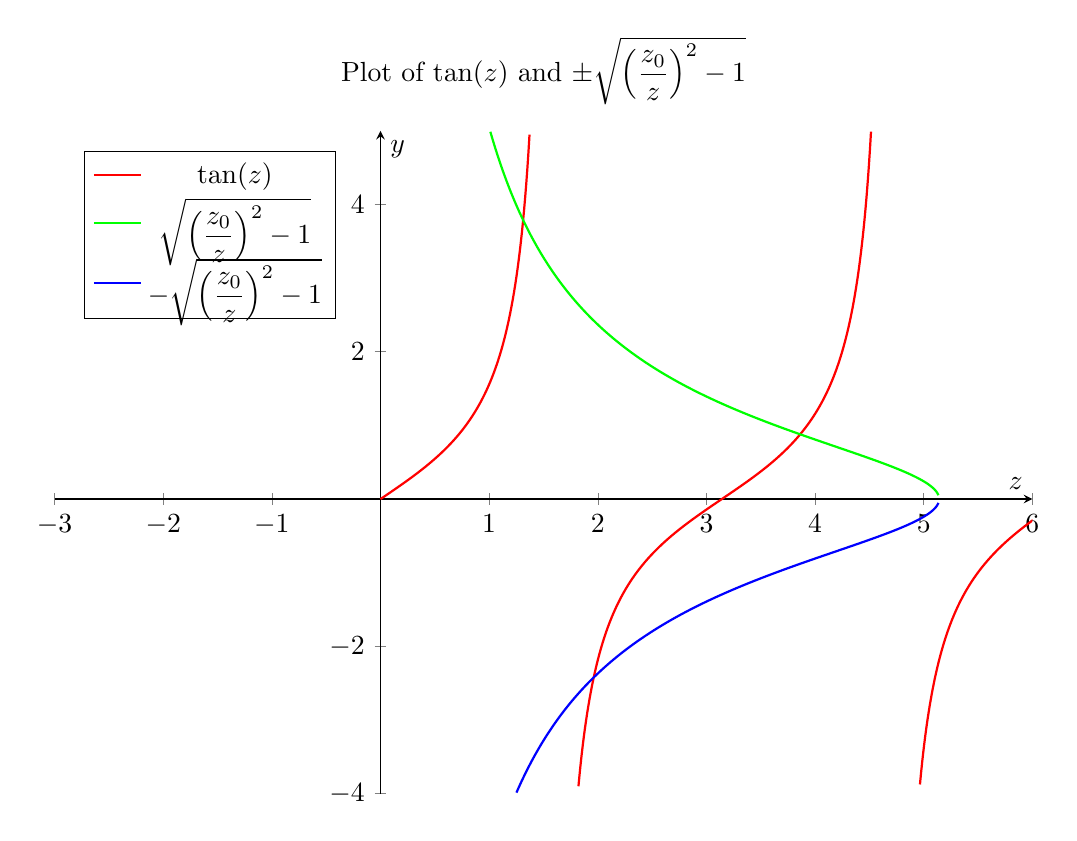
\begin{tikzpicture}
              \begin{axis}[
                      width=14cm, height=10cm,
                      xlabel={$z$},
                      ylabel={$y$},
                      domain=0:6,
                      samples=1000,
                      axis lines=middle,
                      xmin=-3, xmax=6,
                      ymin=-4, ymax=5,
                      restrict y to domain=-4:5,
                      legend entries={$\tan(z)$, $\sqrt{\left(\dfrac{z_0}{z}\right)^2 - 1}$, $-\sqrt{\left(\dfrac{z_0}{z}\right)^2 - 1}$},
                      legend pos=north west,
                      trig format=rad,
                      no markers,
                      title={Plot of $\tan(z)$ and $\pm \sqrt{\left( \dfrac{z_0}{z} \right)^2 - 1}$}
                  ]

                  \def\z0{5.1421638281}

                  \addplot[red, thick, domain=0:10] {tan(x)};
                  \addplot[green, thick, domain=0:10, samples=1000] {sqrt((\z0/x)^2 -1)};
                  \addplot[blue, thick, domain=0:10, samples=1000] {-sqrt((\z0/x)^2 -1)};
              \end{axis}
          \end{tikzpicture}

          \[
              z \approx 1.31266, 3.86258, 1.96234
          \]



\end{enumerate}

\newpage

\bibliographystyle{plain}
\bibliography{references}
\nocite{El-Deeb_PEU-323_Assignments}

\end{document}